\section{Моделирование термического растекания резиста}


\subsection{Аналитический подход}
Моделирование оплавления резиста может быть проведено аналитически на основе подхода, предложенного для моделирования оплавления периодических структур, полученных методом НИЛ~\cite{Leveder_2008, Leveder_2011}. В его основе лежит Фурье-преобразование профиля резиста $h(t)$:
\begin{equation}
	\begin{aligned}
		& h(x, t) = h_0 + \tilde{h}(x, t) \\
		& \tilde{h}(x, t) = \sum_{-\infty}^{+\infty} a_n(t) \exp \left(i n \frac{2 \pi}{\lambda} x\right),
	\end{aligned}
\end{equation}
где $h_0$ -- средняя высота профиля, $\lambda$ -- пространственный период профиля.

Уравнения Навье-Стокса при условии отсутствия проскальзывания и с учетом расклинивающего и Лапласова давления может быть выражено в виде:
\begin{equation}
	\partial_t \tilde{h}-\frac{A}{6 \pi \eta h_0} \partial_x^2 \tilde{h}+\frac{\gamma h_0^3}{3 \eta} \partial_x^4 \tilde{h} = 0,
\end{equation}
где $A$ -- постоянная Гамакера, $\gamma$ -- коэффициент поверхностного натяжения резиста.

Его решение приводит к выражению для времени затухания $n$-й гармоники профиля $\tau_n$:
\begin{equation}
	\frac{1}{\tau_n}=\left(n \frac{2 \pi}{\lambda}\right)^2 \frac{A}{6 \pi h_0 \eta}+\left(n \frac{2 \pi}{\lambda}\right)^4 \frac{\gamma h_0^3}{3 \eta}.
\end{equation}

При выполнении условия $\left(\frac{\displaystyle h_0^2}{\displaystyle \lambda}\right)^2 \ll \frac{\displaystyle A}{\displaystyle \gamma}$ выражение для $\tau_n$ принимает более простой вид:
\begin{equation}
	\tau_n=\frac{3 \eta}{\gamma h_0^3} \times\left(\frac{\lambda}{2 \pi n}\right)^4.
\end{equation}

Результирующий профиль в момент времени $t$ определяется суммой гармоник:
\begin{equation}
	\tilde{h}(x, t)=\sum_{-\infty}^{+\infty} a_n(0) \exp \left(-\frac{t}{\tau_n}+i n \frac{2 \pi}{\lambda} x\right).
\end{equation}

\begin{figure}
	\begin{center}
		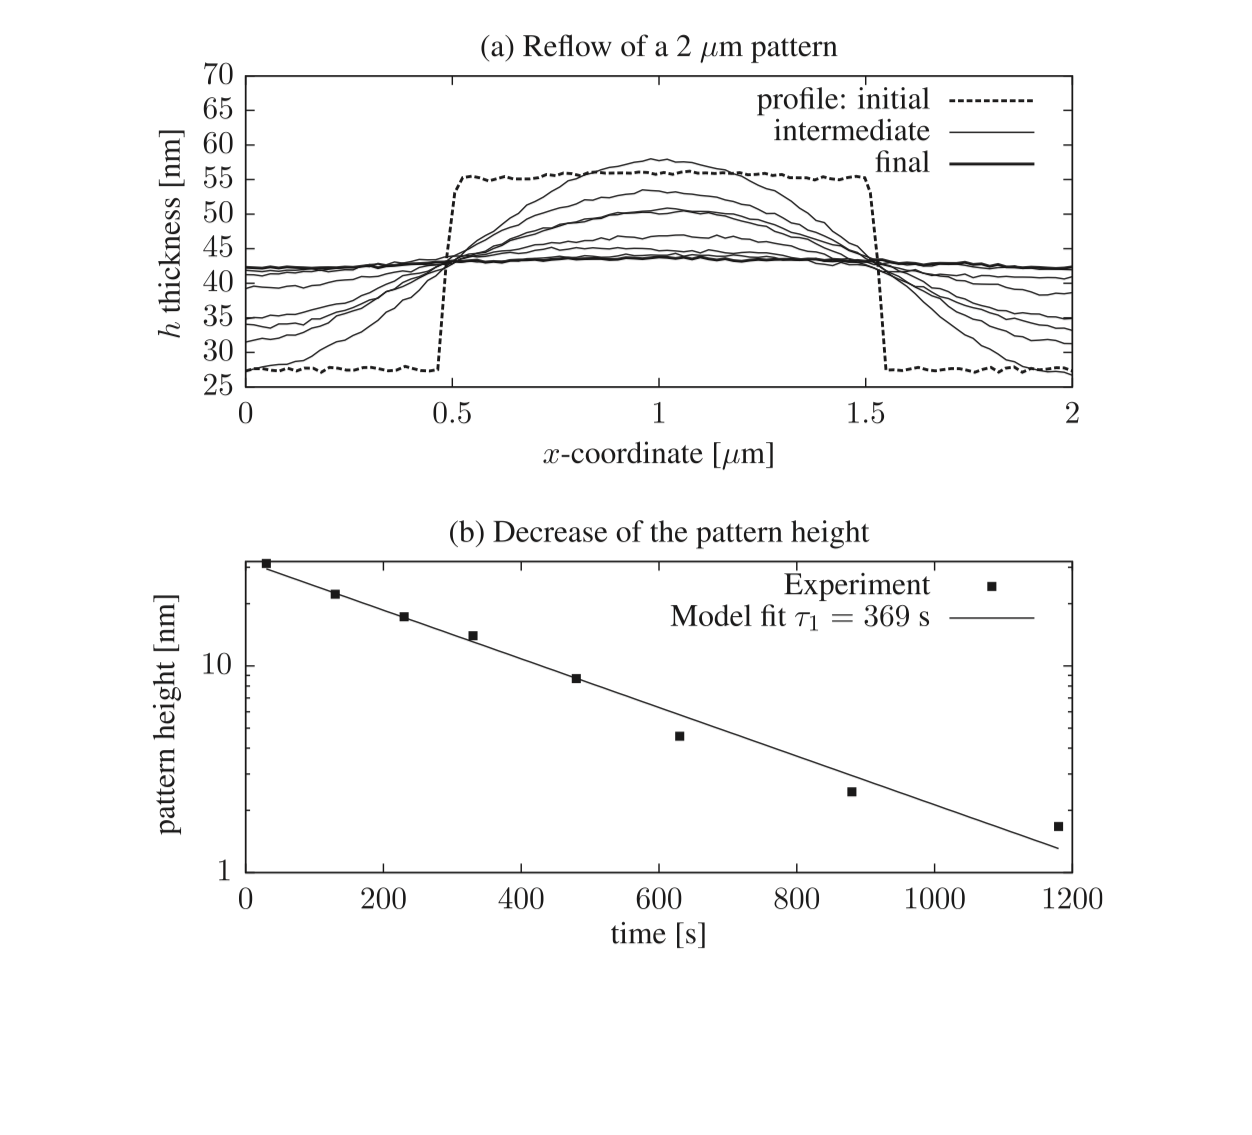
\includegraphics[width=0.6\linewidth]{reflow_analytical}
		\caption{Растекание решетки с периодом 2 мкм, полученной в ПММА методом наноимпринтной литографии~\cite{Leveder_2011}. Нагрев производился при температуре 145 $^\circ$С, время нагрева составляло от 50 до 1200 с: а) 2D профили, полученные методом атомно-силовой микроскопии, б) зависимость от времени высоты профиля решетки (точки) и подгонка линейной функцией (сплошная линия).}
		\label{fig:ferlow_analytical}
	\end{center}
\end{figure}


\subsection{Численный подход}
Второй подход к моделированию растекания профиля резиста основан на использовании численного метода конечных элементов, реализованном в программе \textquotedbl Surface Evolver\textquotedbl{}~\cite{Brakke_SE}. В этом подходе структурные свойства трехмерного объекта задаются свойствами его поверхности, и эволюция формы объекта в различных процессах описываются изменением формы его поверхности. При этом объем внутри поверхности на протяжении процесса эволюции формы поддерживается постоянным. В процессе моделирования поверхность объекта разбивается на треугольные площадки -- грани, задаваемыми тремя узлами -- вершинами, которые, в свою очередь, соединяются ориентированными ребрами~\ref{fig:SE_12}.

В процессе моделирования эволюции формы объекта производится на основе минимизации полной поверхностной энергии. Энергия отдельной грани вычисляется по формуле
\begin{equation}
	E_i=\frac{\gamma_i}{2}\left\|\vec{e}_0 \times \vec{e}_1\right\|,
\end{equation}
где $\gamma_i$ -- коэффициент поверхностного натяжения грани с номером $i$. Сила, действующая на вершину $V_0$ (рис.~\ref{fig:SE_12}), определяется выражением
\begin{equation}
	\vec{F}_{V_0}=\frac{T}{2} \cdot \frac{\vec{e}_1 \times\left(\vec{e}_0 \times \vec{e}_1\right)}{\left\|\vec{e}_0 \times \vec{e}_1\right\|}.
\end{equation}

При моделировании растекания двумерных структур в резисте последние представляются в виде фигуры бесконечной протяженность. При этом моделирование проводится для участка фигуры конечной длины с использованием зеркальных граничных условия на краях участка~\ref{fig:SE_3}. Таким образом, возникают три возможных типа граней -- грани на границе полимер/вакуум ($p$), грани на границе полимер/подложка ($ps$) и боковые (зеркальные) грани ($m$). Полная энергия поверхности $E_{tot}$ вычисляется по формуле
\begin{equation}
	E_{tot}=E_p-(E_{p s}+E_m),
\end{equation}
где 
\begin{equation}
	E_x = \sum_{i} E_{x,i}, \hspace{0.5em} x = p, ps, m
\end{equation}

\begin{figure}
	\begin{minipage}{0.55\textwidth}
		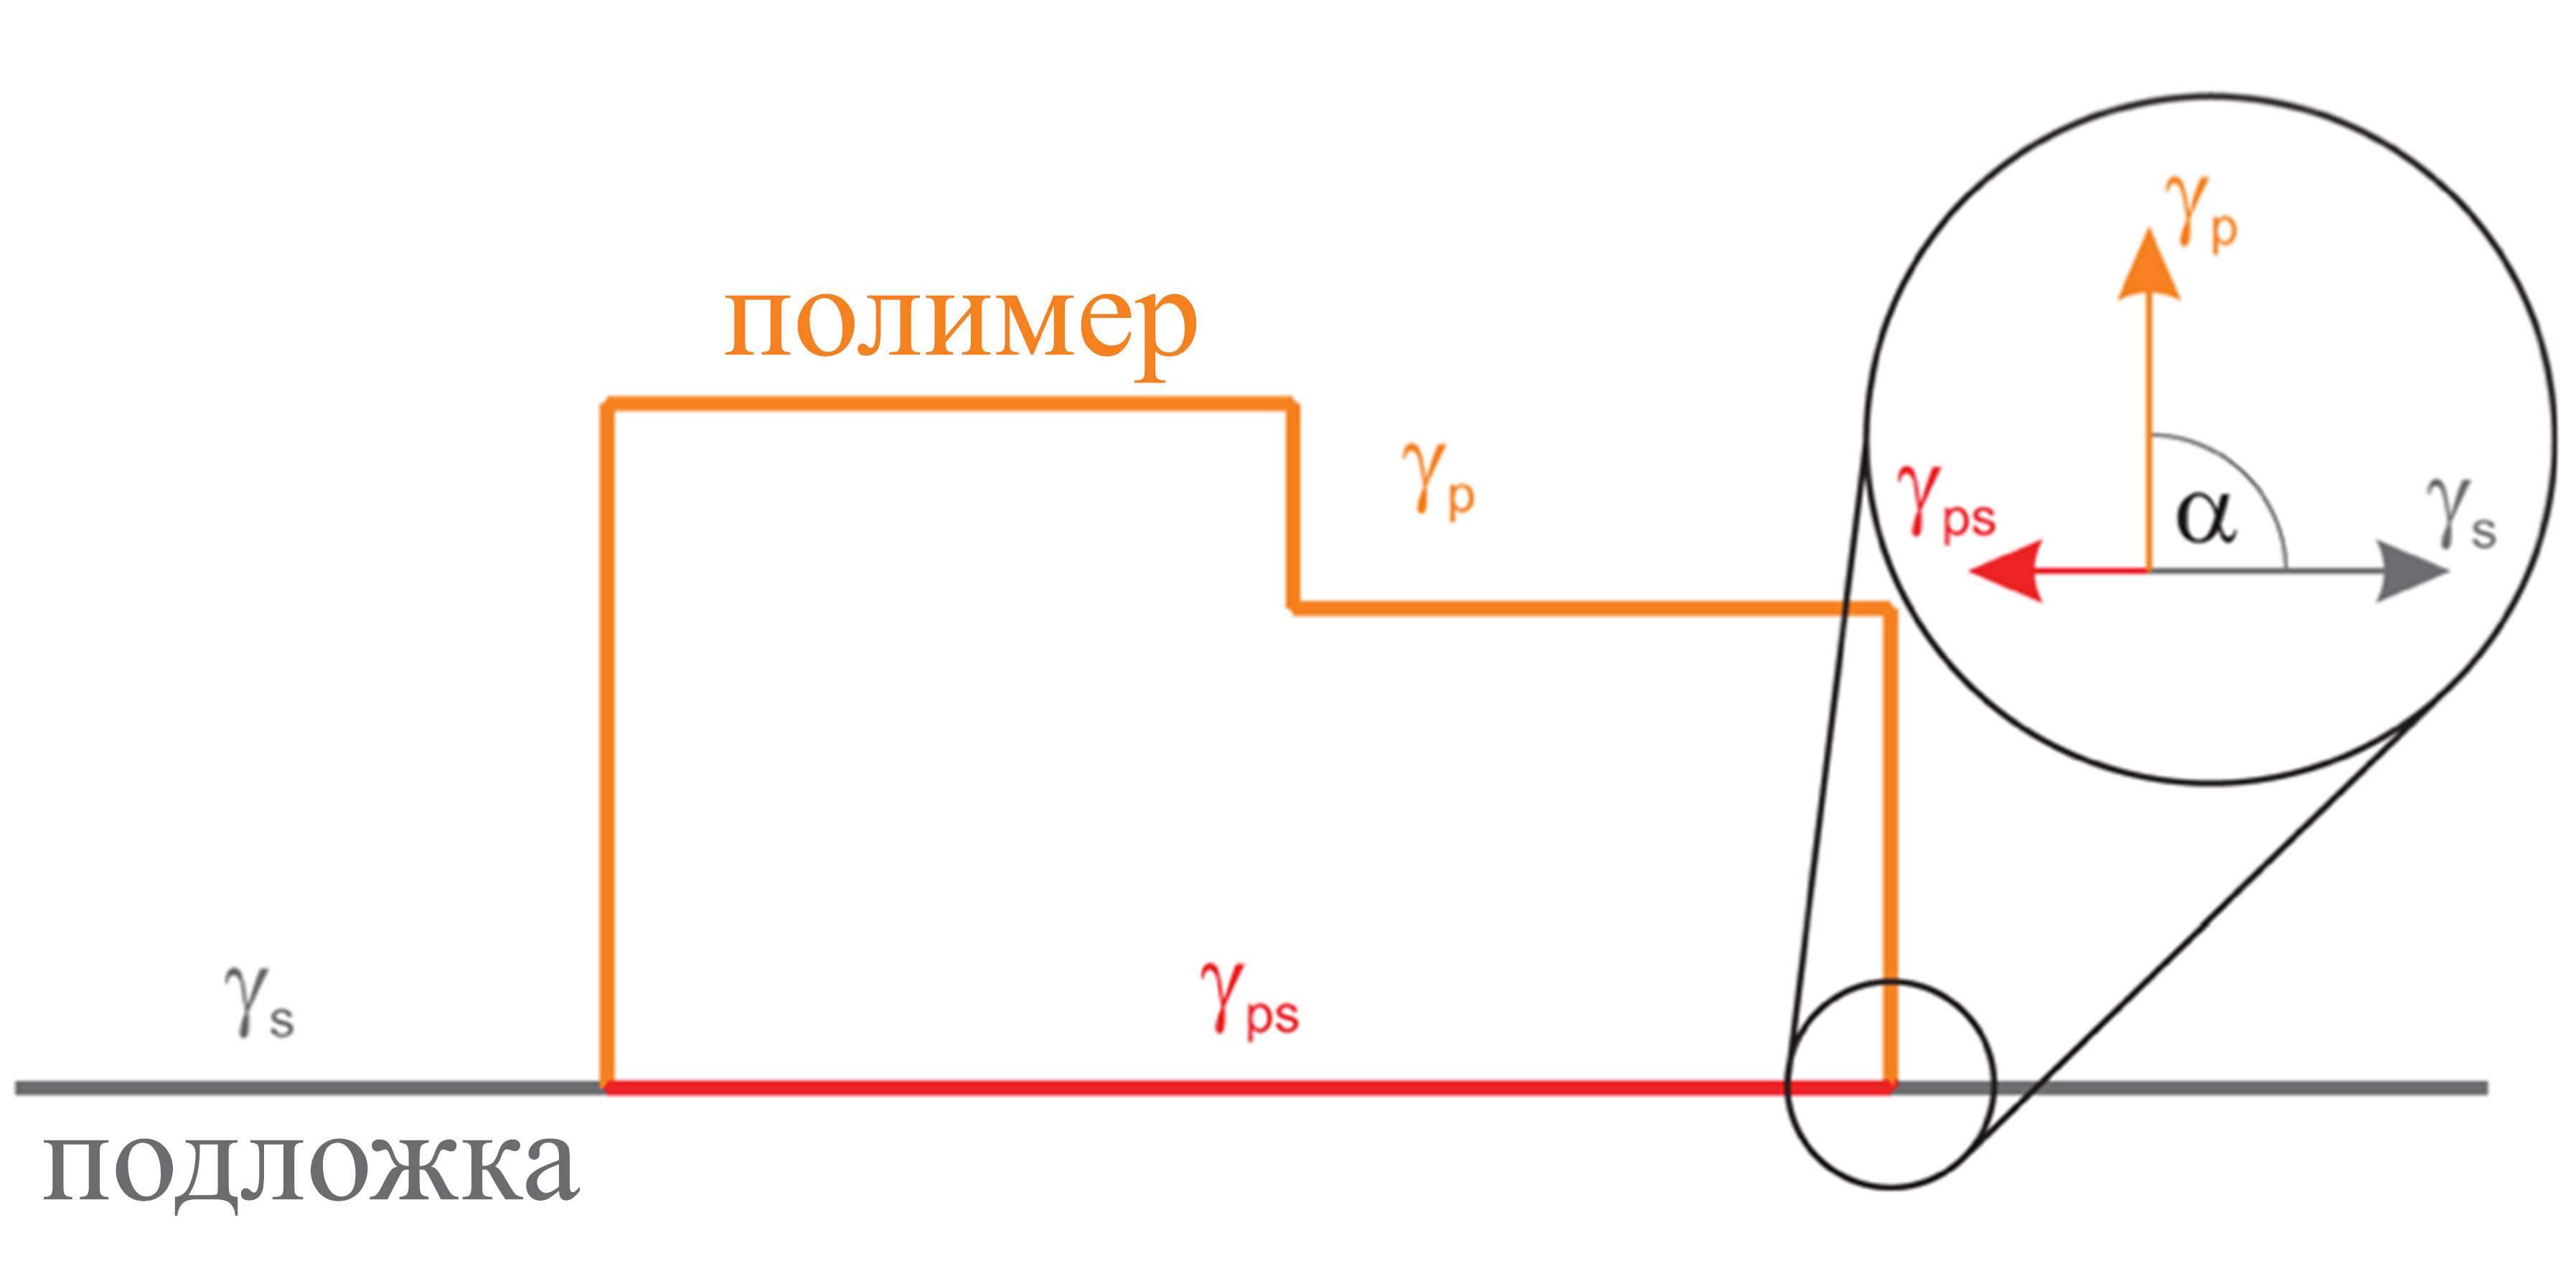
\includegraphics[width=\linewidth]{SE_1}
	\end{minipage}
	\begin{minipage}{0.4\textwidth}
		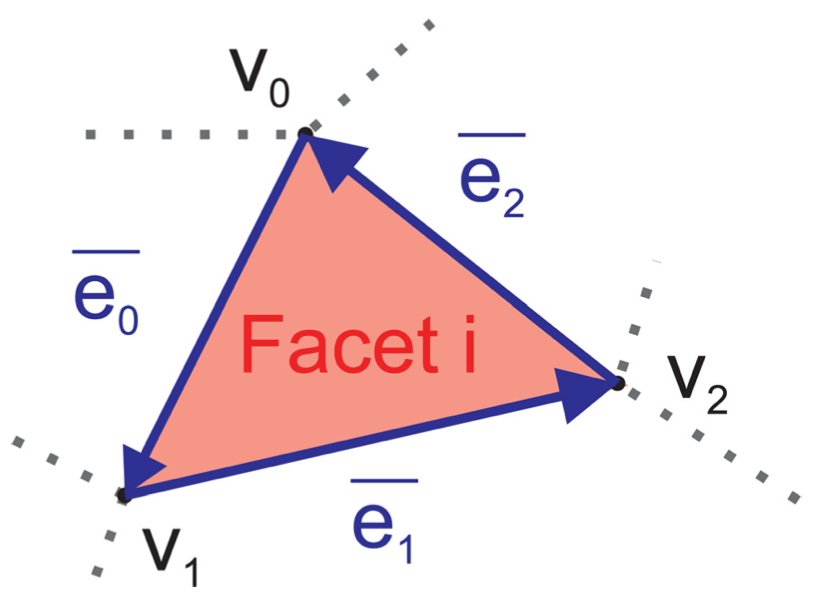
\includegraphics[width=\linewidth]{SE_2}
	\end{minipage}
	\caption{Схематическое изображение поверхности в программе \textquotedbl Surface Evolver\textquotedbl{}}.
	\label{fig:SE_12}
\end{figure}

В работах по использованию программы \textquotedbl Surface Evolver\textquotedbl{} для моделирования растекания слоя ПММА моделирование проводилось в режиме нормализации площади, использующимся для реалистичного описания движения под действием сил поверхностного натяжения. В этом режиме при вычислении силы, действующей на вершину, учитывается площадь всех граней, окружающих вершину. Поскольку каждая из граней задается тремя вершинами,
сила, действующая на каждую из вершин грани, будет пропорциональна отношению площади грани к 1/3 площади всех граней, окружающих данную вершину ($A$):
\begin{equation}
	\vec{F}_{norm} = \frac{\vec{F}}{A/3} = \frac{3\vec{F}}{A}.
\end{equation}

Связь силы, действующей на вершину, со скоростью движения вершины в процессе эволюции поверхности описывается коэффициентом подвижности вершины $m$:
\begin{equation}
	\vec{v} = \vec{F}_{norm} \cdot m = \frac{\vec{F}}{A/3} \cdot m.
\end{equation}

Наконец, смещение вершины определяется формулой
\begin{equation} \label{eq:SE_delta}
	\boldsymbol{\delta} = \vec{v} \cdot scale,
\end{equation}
где $scale$ -- величина, аналогичная времени.

Следует отметить, что в исходном виде данный метод является чисто математической моделью, на что указывает характер зависимости~\ref{eq:SE_delta}, а также использование величины $scale$ вместо привычного \textquotedbl физического\textquotedbl{} времени.
\begin{figure}[t!]
	\begin{center}
		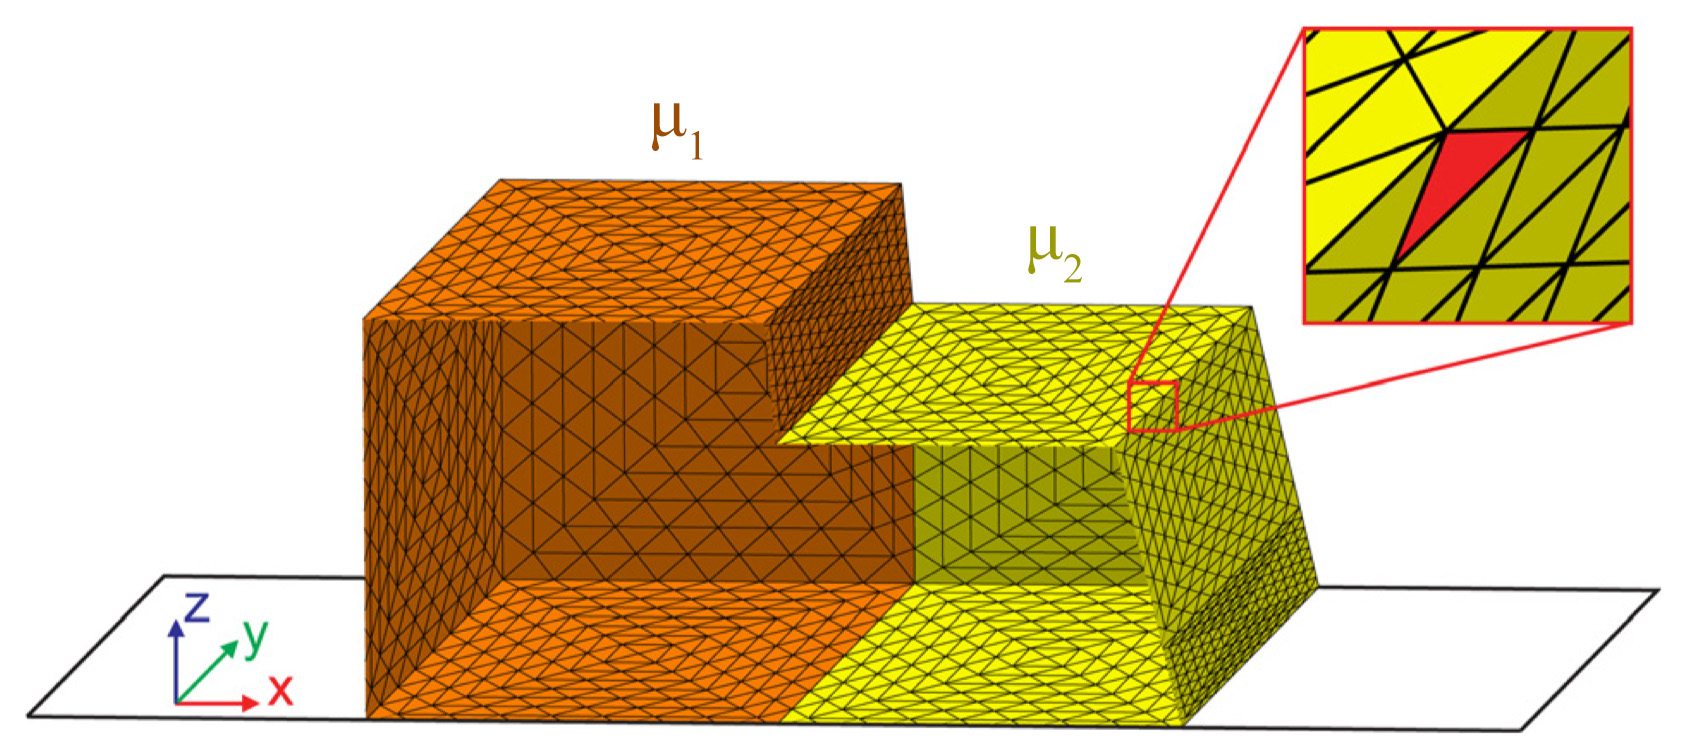
\includegraphics[width=0.9\linewidth]{SE_3}
		\caption{Модель поверхности образца, полученного методом полутоновой литографии, заданная в программе \textquotedbl Surface Evolver\textquotedbl{}~\cite{Kirchner_reflow}.}
		\label{fig:SE_3}
	\end{center}
\end{figure}





